\chapter{Diferenças entre Bancos de Dados Relacionais e NoSQL}

O armazenamento a a manipulação de dados tem sido um importante foco da computação desde o seu nascimento, tendo os bancos de dados suas raízes ja na década de 60, principalmente em aplicações médicas e científicas~\cite{neufeld1986database}, e em 1970, Edgar Codd propos uma nova forma de armazenamento de dados, que ficou conhecida como modelo de dados relacionais (\emph{relational model of data})~\cite{codd1970relational}. 

\section{Bancos de Dados Relacionais}
    Podemos definir um banco de dados relacional como um conjunto de dados que se relacionam entre si e que são armazenados de forma persistente, podendo ser recuperados quando necessario. Os dados são armazenados em tabelas, que são organizadas por colunas, que definem uma categoria de um dado, e por linhas, que representam a instância de um dado~\cite{leavitt2010nosql}. A popularização desse modelo em virtude de suas características de persistência, concorrência e integração entre múltiplas aplicações, o transformou no modelo padrão de armazenamento computacional, principalmente em ambientes empresarias~\cite{pramod}. Outra questão de importância em bancos de dados computacionais é a não necessidade que o usuario tem de conhecer como esses dados são armazenados, o que foi possível com o uso dos chamados Sistemas Gerenciadores de Bancos de Dados (SGBDs)~\cite{jan}.
    
    Outras opções surgiram ao longo dos anos, como os bancos orientados a objetos ou bancos XML. Nenhum deles, entretanto, conseguiu competir com o modelo ja tradicional de dados relacionais.~\cite{pramod} Nos últimos anos, entretanto, o modelo conhecido como NoSQL vem surgindo como essa alternativa.
    
    Bancos de Dados relacionais tem como um de seus requisitos a existência de chaves primarias, colunas que que identificam unicamente cada linha, ou registro, de uma tabela. Um banco de dados relacional necessita de três informações para recuperar um dado específico: o nome da tabela, o nome da coluna e a chave primaria do registro que esta sendo buscado \cite{jan}.

\subsection{Propriedades ACID}
	Interações com bancos de dados relacionais tradicionais são feitas por meio de transações, que podem ser definidas como operações de leitura e escrita que devem ocorrer de forma independente umas das outras~\cite{dmsbook}. Para garantir que isso ocorra, um SGBD deve prover as seguintes propriedades, conhecidas como propriedades ACID~\cite{haerder}:
	\begin{itemize}
	\item \textbf{Atomicidade}, onde uma determinada transação deve ser feita em sua totalidade, ou seja, todas as operações de que dela fazem parte devem ser bem sucedidas.
	\item \textbf{Consistência} diz que após cada transação, o estado do banco permanece consistente ao seu modelo.
	\item \textbf{Isolamento} garante que cada transação é executada independentemente de outras que estejam ocorrendo em concorrência.
	\item \textbf{Durabilidade} que define que o resultado de uma transação bem sucedida é persistido no banco, mesmo na eventualidade de falhas no sistema.
	\end{itemize}

	Essas propriedades, ao mesmo tempo que garantem a validade do esquema e dos dados em um banco, sacrificam desempenho e disponibilidade, características importantes em varias aplicações atuais~\cite{foxcluster}.

\subsection{Normalização}
	Uma pratica comum e recomendada no projeto de bancos de dados relacionais é a normalização. O processo de normalização segue regras conhecidas como formas normais, onde cada forma normal representa um incremento desse conjunto de regras \cite{jan}. 
	Existem pelo menos seis formas normais, mas na maioria dos casos um banco é considerado bem projetado quando cumpre as exigências da terceira forma normal (3FN).

\subsection*{Primeira Forma Normal}
	Uma tabela esta na primeira forma normal (\textbf{1FN}) se cada tabela esta organizada por colunas e linhas, com cada linha possuindo uma chave primaria única que a identifica. 
	Além disso cada campo deve possuir apenas valores atômicos. Ou seja, cada coluna deve guardar apenas uma informação, não podendo existir listas ou conjuntos de valores dentro de uma mesma coluna de uma linha.

\subsection*{Segunda Forma Normal}
	Uma tabela esta na segunda forma normal (\textbf{2FN}) quando, além de obedecer à primeira forma normal, possui todos atributos não-chave funcionalmente dependentes da chave primaria. Dependência funcional é definida como uma relação entre dois atributos tal que para cada valor único do atributo A, existe apenas um valor do atributo B associado a ele~\cite{jan}. Em outras palavras, uma coluna não pode depender apenas de parte da chave primaria, ou seja, se uma tabela não possui chave primaria composta e esta na primeira forma normal, ela também esta na segunda forma normal.
	
\subsection*{Terceira Forma Normal}
	Uma tabela esta na terceira forma normal (\textbf{3FN}) quando, além de obedecer à segunda forma normal, não apresenta dependências transitivas, ou seja, cada atributo não-chave não pode ser determinado, ou dependente, de outro atributo não-chave. 

\section{Bancos NoSQL}
    O rapido crescimento no volume de dados nos últimos anos, principalmente após a bolha da Internet na década de 90~\cite{pramod}, tras uma necessidade de certa mudança em relação ao modelo tradicional. Modelos relacionais possuem diversas vantagem ja citadas, porém restrições como propriedades ACID e normalização, levam ao surgimento de problemas quando precisamos aplica-los nesse domínio recente de expansão dos dados, por apresentarem problemas de escalabilidade, complexidade dos dados e rigidez em seus esquemas~\cite{leavitt2010nosql}. 
    
    Isso levou ao surgimento de um movimento em direção ao novo paradigma denominado NoSQL. O termo foi utilizado pela primeira vez em 1998 para denominar um banco de dados que omitia o uso de SQL, o \emph{Strozzi NOSQL}. A definição atual, porém, tem suas bases em uma reunião, conhecida como \emph{NoSQL Meetup} realizada em 2009 em São Franscisco, Estados Unidos. Organizada por Johan Oskarsdon, criador do Last.fm, nela foram discutidas formas mais eficientes e baratas de organização dos dados, como as ja sugeridas em publicações anteriores, como o Google Bigtable em 2006~\cite{bigtable}, e Amazon's Dynamo em 2007~\cite{dynamo, chrisnosql}.
\subsection{Definição e Características}
Apesar do termo não tem uma definição precisa e universalmente aceita, sendo geralmente descrito como \emph{Not Only SQL}, bancos NoSQL em geral são caracterizados, mas não definidos, como sendo não relacionais, sem esquema bem definido, distribuidos e tolerantes a falhas~\cite{pramod}. Buscam um processamento de dados rápido e de forma eficiente, evitando a rigidez dos bancos tradicionais. 
	Entre as razões e vantagens dos bancos NoSQL podemos citar~\cite{chrisnosql}:
    \begin{itemize}
    \item \textbf{Evitar complexidade desnecessária}: Bancos relacionais costumam aderir às já citadas propriedades ACID, além de serem restritos em seu esquema de dados. Bancos NoSQL costumam ignorar ou relaxar essas restrições a fim de obter um melhor desempenho.
    \item \textbf{Alto rendimento}: Bancos NoSQL surgiram da necessidade e armazenamento e processamento de um cada vez maior volume de dados, e por isso são construídos objetivando um desempenho melhor, em aplicações específicas, do que de bancos tradicionais.
    \item \textbf{Alta escalabilidade}: Bancos relacionais podem ser escalados verticamente com a utilização de equipamentos poderosos e caros, e uma operação distribuida costuma ser mais complexa devido à forma de armazenamento de seus dados~\cite{leavitt2010nosql}. Bancos NoSQL foram pensados para execução em um sistema de \emph{clusters}, o que facilita a sua escalabilidade horizontal e reduz a necessidade de um hardware mais caro e específico, podendo ser utilizado em \emph{hardwares} mais simples. 
    \item \textbf{Alta disponibilidade}: Devido à possibilidade de escalabilidade horizontal, bancos NoSQL podem distribuir sua operação em diversos nós de um \emph{cluster}, o que possibilita acesso simultâneo por um grande número de usuários, mesmo que não seja possível acessar algum desses nós. 
    \item \textbf{\emph{Open source}}: SGBDs tradicionais costumam possuir licenças pagas, gerando um custo financeiro alto, principalmente quando executados em múltiplas maquinas~\cite{pramod}. NoSQLs costumam seguir licenças \emph{open source}, podendo reduzir significativamente os gastos da aplicação. 
\end{itemize}

\subsection{Teorema CAP}
\label{sec:cap}
	Em 2000 Eric Brewer, pesquisador na \emph{University of California}, propõs o teorema CAP, que define limitações em sistemas distribuidos. O teorema define que podemos garantir somente duas das seguintes três propriedades em um determinado sistema: Consistência (\emph{Consistency}) , Disponibilidade (\emph{Availability}) e Tolerância a partições (\emph{Partition-resilience})~\cite{brewer}. Essas propriedades podem ser definidas como:
    \begin{itemize}
	\item \textbf{Consistência} define que todos os nós possuem os mesmos dados em qualquer dado instante, e um pedido de leitura em qualquer desses nodos garante o dado mais atual possível do sistema.
    \item \textbf{Disponibilidade} garante é sempre possível ler e gravar dados em um nodo dado que ele esta acessível. 
    \item \textbf{Tolerância a partições} garante que o sistema ira continuar funcionando mesmo na hipótese de eventuais falhas de comunicação entre os nodos.
	\end{itemize}
	
    Essas propriedades podem ser agrupadas da seguinte forma e obtendo os seguintes resultados:
    \begin{itemize}
    \item \textbf{CA} são sistemas distribuídos cujos nós estejam em uma mesma partição de rede.
    \item \textbf{CP} são sistemas que, em caso de falha em pelo menos um dos nós, ficam indisponíveis até sua total recuperação. Bancos de Dados que seguem as propriedades ACID costumam seguir esse padrão.
    \item \textbf{AP} são sistemas que devem permanecer em funcionamento mesmo durante uma eventual falha em um ou mais de seus nós, mesmo que isso resulte em dados não atualizados durante consultas. Sistemas NoSQL costumam seguir esse padrão.  
	\end{itemize}
    
    Sistemas distribuídos, entretanto, por estarem sempre sujeitos a falhas de rede~\cite{deutsch}, não podem ignorar a Tolerância a Falhas, tendo de fazer uma escolha entre Consistência e Disponibilidade~\cite{brewer12years}.
    
    A figura \ref{fig:capnosql} ilustra as diferentes combinações das propriedades CAP e exemplos de bancos de dados que as utilizam.
    

\begin{figure}[!htb]
\centering
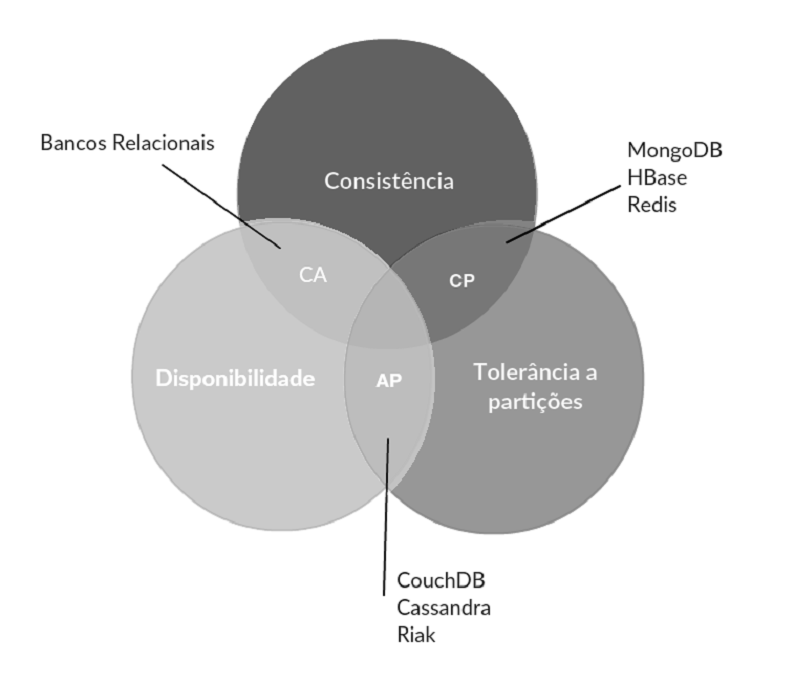
\includegraphics[width=0.65\textwidth]{figuras/cappb.png}
\caption{Propriedades CAP e exemplos. Adaptado de ~\cite{blograshid}}
\label{fig:capnosql}
\end{figure}

\subsection{BASE}
    Em um ambiente distribuido, escabalibilidade, resiliência e velocidade são mais importantes do que consistência imediata e segurança quanto à veracidade dos  dados, não sendo necessaria a aderência total às propriedades ACID ja citadas~\cite{neo4j_acidbase}. Além disso, de acordo com o \textbf{Teorema CAP}, um banco que aceite particionamento não pode possuir alta disponibilidade e consistência simultâneamente. Essa necessidade, tanto de performance quanto de disponibilidade, levou à criação do acrônimo \textbf{BASE}, \emph{\textbf{B}asically \textbf{A}vailable} (Basicamente Disponível), \emph{\textbf{S}oft State} (Estado Leve) e \emph{\textbf{E}ventual Consistency} (Consistência Eventual)~\cite{foxcluster}. 
    
    Enquanto um banco \textbf{ACID} é pessimista, requerendo que cada operação mantenha a consistência do banco como um todo, \textbf{BASE} segue uma visão otimista, entendendo que dados serão eventualmente consistentes.
    
    Sistemas distribuídos costumam manter cópias de dados em varias maquinas em um \emph{cluster} para aumentar a sua disponibilidade, e quando um desses dados é atualizado em uma dessas maquinas é natural que haja um intervalo de tempo até que todas essas cópias sejam atualizadas.

\subsection{Modelos NoSQL}
Bancos de dados NoSQL possuem padrões de modelos de dados, que compartilham certas características em comum e servem a determinadas aplicações específicas, podendo alguns bancos serem classificados em mais de uma categoria. A tabela \ref{tab:modelosnosql} lista os quatro modelos atuais e alguns bancos de dados que se enquadram em cada um deles.

~\begin{table}[]
\centering
\caption{Modelos de Bancos NoSQL}
\label{tab:modelosnosql}
\begin{tabular}{ll}
\textbf{Modelo de Dados}     & \textbf{Exemplo de bancos de dados}      \\ \hline
Chave-Valor         & Project Voldemort               \\
                    & Riak                            \\
                    & Redis                           \\
                    & BerkeleyDB                      \\ \hline
Documentos          & CouchDB                         \\
                    & MongoDB                         \\
                    & OrientDB                        \\ \hline
Famílias de colunas & Cassandra                       \\
					& Hypertable                      \\
                    & HBase                           \\ \hline
Grafos              & Neo4j \\
                    & OrientDB                        \\
                    & Infinite Graph                 
\end{tabular}
\end{table}

\subsection*{Chave-Valor}
Bancos com armazenamento em chave-valor existem a muito tempo, como \emph{Berkeley DB}, mas ganharam importância no meio NoSQL a partir do Amazon DynamoDB e do Google BigTable~\cite{chrisnosql}.

Consiste basicamente em uma tabela \emph{hash}, sendo o acesso aos dados realizado por meio de uma chave primaria, assim como ocorre em \emph{maps} e dicionarios.  Esses bancos são completamente livres de esquema e suas operações se resumem a consultar o valor a partir de uma chave, inserir um valor para uma chave ou deletar uma chave e seu valor do banco~\cite{nosqleval}. O valor armazenado em geral pode representar qualquer tipo de objeto, como uma \emph{string} ou um \emph{BLOB}, não sendo necessária que exista qualquer relação entre diferentes registros, ficando a aplicação responsável pelo seu tratamento. 

Esses bancos favorecem escalabilidade sobre consistência, e por isso em geral não possuem ferramentas mais poderosas de consulta e analise de dados~\cite{chrisnosql}.

Atualmente temos como exemplos de bancos chave-valor: \emph{Riak}, \emph{Redis}, \emph{Berkeley DB} e \emph{Project Voldemort}.

\subsection*{Documentos}
Bancos orientados a documentos armazenam seus dados em forma de documentos, podendo esses terem formato \emph{XML}, \emph{JSON}, \emph{BSON}, etc~\cite{pramod}. Podem ser vistos como a sequência natural do armazenamento por chave-valor, ainda fazendo o armazenamento por meio de um par chave-valor, mas utilizando uma estrutura mais rica para armazenamento dos dados ao armazenar um documento na parte do valor~\cite{chrisnosql}. Cada um desses documentos pode ter certa semelhança uns com os outros, mas não necessitam possuir a mesma estrutura, o que permite uma grande flexibilidade no esquema do banco.

A seguir temos um exemplo de dois documentos. Apesar de parecidos, eles possuem certas diferenças, o que gera essa grande flexibilidade do modelo orientado a documentos.

\begin{lstlisting}
{
  "clienteid" : "f6a6fs86fa",
  "cliente" :
  {
    "primeironome" : "Pedro",
    "sobrenome" : "Silva", 
    "gosta" : ["Leitura", "Viagem"]
  }
  "endereco" : 
  {
    "estado" : "Sao Paulo",
    "cidade" : "Guarulhos"
  }
}

{
  "clienteid" : "ga9s8g8fe",
  "cliente" :
  {
    "primeironome" : "Maria",
    "sobrenome" : "Costa", 
    "gosta" : ["Esportes"]
  }
  "ultimaCompra" : "12/11/2015"
}
\end{lstlisting}

Esses documentos não são opacos à aplicação, seu conteúdo pode ser consultado diretamente, com consultas diretas em atributos de seus registros. Isso permite a manipulação de estruturas mais complexas, que ainda assim não possuem nenhuma restrição de esquema, sendo facil a inserção de novos documentos ou a modificação dos documentos ja armazenados. Devido à essa flexibilidade, são recomendados para integração de dados e migração de esquemas~\cite{nosqleval}. 

Como exemplos de bancos orientados a documentos podemos citar o \emph{CouchDB}, \emph{MongoDB} e \emph{OrientDB}.

\subsection*{Colunas}
Bancos de Dados colunares tem sua influência no \emph{Google BigTable}~\cite{bigtable}, e armazenam seus dados em famílias de colunas que são associadas a uma chave de linha. Cada uma dessas famílias de colunas pode possuir varias colunas, e são consideradas dados relacionados que podem ser acessados ao mesmo tempo~\cite{pramod}. 

O Cassandra possui ainda o conceito de super colunas, que pode ser visto como um agrupamento de colunas que pode ser armazenado dentro de uma família de colunas~\cite{pramod}.

Colunas e linhas podem ser adicionadas a qualquer momento, o que gera uma flexibilidade bem maior em relação aos esquemas em geral fixos dos bancos de dados relacionais.  Entretanto, famílias de colunas em geral devem ser predefinidas, situação menos flexível que a encontrada nos modelos de chave-valor ou de documentos~\cite{nosqleval}.  

Como exemplo de bancos orientados a colunas temos o \emph{HBase} e \emph{Hypertable}, que são implementações \emph{open source} do BigTable, e o \emph{Cassandra}.


\subsection*{Grafos}
Diferente dos bancos relacionais e dos ja citados modelos NoSQL vistos, um banco de dados em grafos é especializado em dados altamente conectados. São ideias para aplicações que realizam consultas baseadas em relações~\cite{nosqleval}.
Esse modelo realiza o armazenamento por meio de entidades e os relacionamentos entre essas entidades. Entidades podem ser vistas como nós e os relacionamentos como as areas de um grafo~\cite{pramod}. Esses nós podem possuir propriedades dos objetos que representam, assim como as áreas, que podem possuir atributos do relacionamento e além disso possuem significância em sua direção.

Consultas nesse tipo de modelo são realizadas percorrendo o grafo. Isso possui como vantagem a possibilidade de se modificar a forma que se camanha nesse grafo, sem ser necessarias mudanças em sua estrutura de nós e relações~\cite{pramod}.

Uma diferença importante dos bancos orientados a grafos em relação aos modelos anteriores é o seu suporte menor a sistemas distribuidos, não sendo geralmente possível a distribuição dos nós em diferentes servidores~\cite{pramod}.

Como exemplos desse modelo podemos citar o \emph{Neo4J}, o \emph{Infinite Graph} e o \emph{OrientDB}.